\fancychapter{mmWave Simulation Plots}
\label{ap:mmWave_simulation_plots}

All plots in this appendix refer to mmWaves. 

The throughput is higher, which is expected if the SINRs are higher as a result of more directive transmissions (more gain, less interference).

\imagecapcontrol{Appendices/mmWave results/mu_throughput_secs_26.0ghz.pdf}{UE bit rates, instantaneous and averaged over the last 200 ms (GoP duration).}{fig_mu_bitrates2}{.73}{-3mm}

The graphs of the SINR, in Figure \ref{fig_mu_sinr2}, and the signal and interference powers, in Figure \ref{fig_mu_pow2}, are consistent. However, UE 0 and UE 2 have different shapes than the same UEs in lower frequency, while UE 1 and UE 3 have the same. This may be due to different beam shapes. 

The MCSs in Figure \ref{fig_mu_mcs2}, much like the SINRs, are consistently higher in mmWaves than in lower frequencies.

The BLERs in Figure \ref{fig_mu_bler2} are very similar to lower frequencies. Figure \ref{fig_mu_olla2} that shows the OLLA parameter correlated with the BLER is also consistent.

Figure \ref{fig_mu_lat2} shows a considerable better performance with respect to latency than 3.5 GHz. More concretely, now 3 out of 4 users have 0\% drop rate. This makes sense since all SINRs are higher. Given a better channel quality, the performance in terms of throughput and latency expectedly improves.

\imagecapcontrol{Appendices/mmWave results/sinr_secs_26.0ghz.pdf}{SINR, estimated before transmission and experienced during transmission.}{fig_mu_sinr2}{.73}{-3mm}

\imagecapcontrol{Appendices/mmWave results/pow_vs_inter_secs_26.0ghz.pdf}{Received Signal and Interference Powers.}{fig_mu_pow2}{.73}{-1mm}


\imagecapcontrol{Appendices/mmWave results/mcs_secs_26.0ghz.pdf}{MCS index used by each UE in every transmission.}{fig_mu_mcs2}{.73}{-3mm}


\imagecapcontrol{Appendices/mmWave results/running_bler_secs_26.0ghz.pdf}{All time BLER average in a multi-user scenario.}{fig_mu_bler2}{.73}{-3mm}



\begin{center}

    \hfill 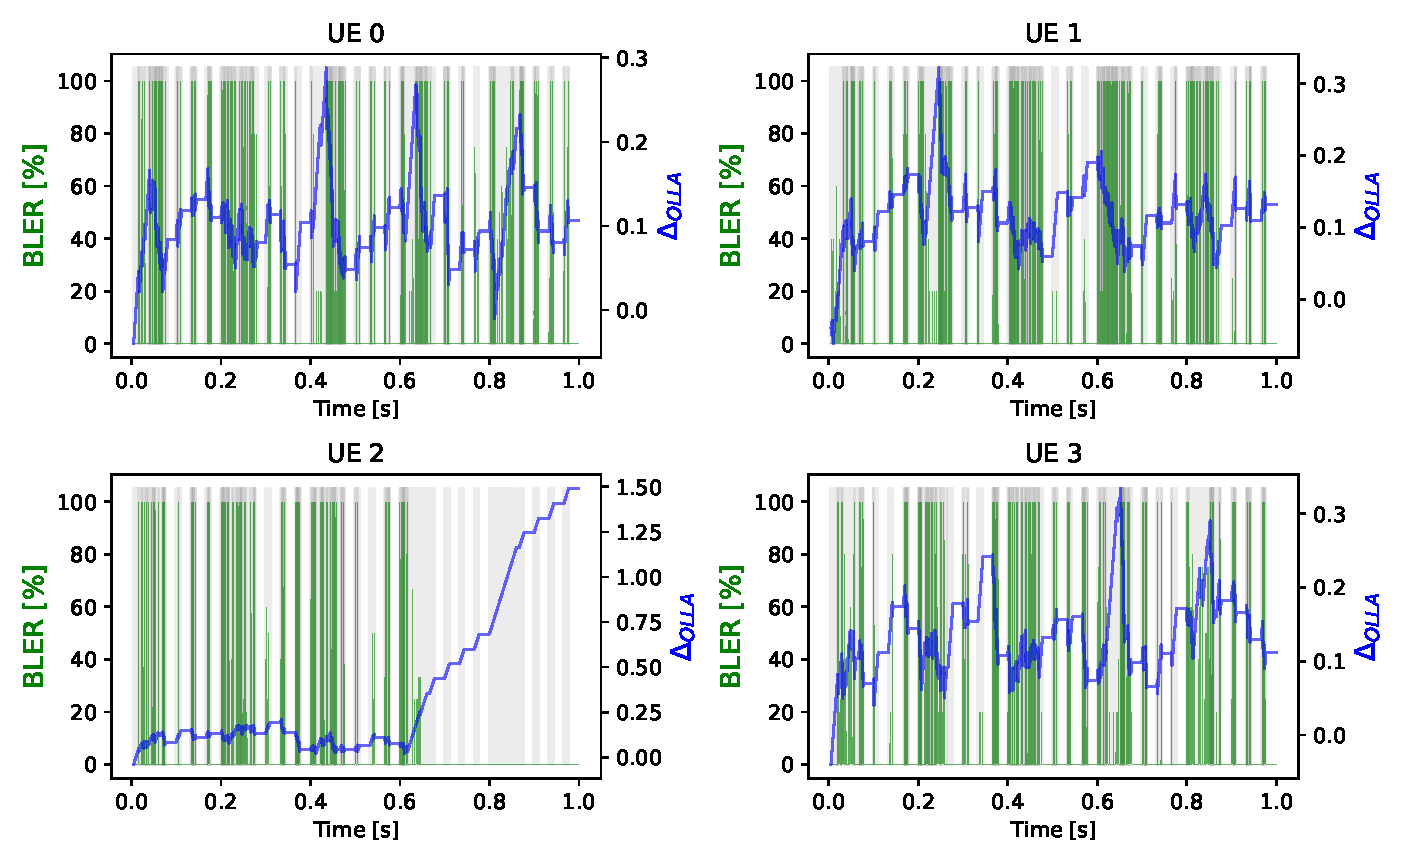
\includegraphics[scale = .59]{Appendices/mmWave results/olla_secs_26.0ghz.pdf}
    \captionsetup{type=figure} 
    \vspace{-3mm}   
    \caption{Link adaptation parameter variation with the instantaneous \acs{BLER}. Grey zones mark when the UE has active transmissions.}			
    \label{fig_mu_olla2}
    
\end{center}



\imagecapcontrol{Appendices/mmWave results/lat_drop_rate_secs_26.0ghz.pdf}{Packet latencies and drop-rates for all UEs with I-frame marking.}{fig_mu_lat2}{.65}{-3mm}


